\documentclass{beamer}

\usepackage[czech]{babel}
\usepackage[utf8]{inputenc}
\usepackage{times}
\usepackage[T1]{fontenc}

\mode<presentation>
{
  \usetheme{Warsaw}
  \usecolortheme{crane} 
}

\setbeamertemplate{footline}{
  \leavevmode%
  \hbox{%
  \begin{beamercolorbox}[wd=.333333\paperwidth,ht=2.25ex,dp=1ex,center]{author in head/foot}%
    \usebeamerfont{author in head/foot}\insertshortauthor
  \end{beamercolorbox}%
  \begin{beamercolorbox}[wd=.333333\paperwidth,ht=2.25ex,dp=1ex,center]{title in head/foot}%
    \usebeamerfont{title in head/foot}\insertshortsubtitle
  \end{beamercolorbox}%
  \begin{beamercolorbox}[wd=.333333\paperwidth,ht=2.25ex,dp=1ex,center]{date in head/foot}%
    \usebeamerfont{date in head/foot}\insertframenumber/6
  \end{beamercolorbox}}%
  \vskip0pt%
}

\title{Urychlení metod k-means a mean-shift pomocí 3D akcelerační karty}
\subtitle{Projekt do předmětu GMU (pr05)}
\author[Martin Šimon \& Pavel Širůček]{Martin Šimon \& Pavel Širůček}
\institute{Vysoké učení technické v Brně - Fakulta informačních technologií}
\date{}

\begin{document}

\begin{frame}[plain]
  \titlepage 
\end{frame}
\addtocounter{framenumber}{-1}


\begin{frame}{K-means a mean-shift}
  \begin{itemize}
    \medskip
    \item Metody pro shlukování - použity pro segmentaci obrazu či kvantizaci barev
    \medskip
    \item Paralelizace algoritmů (případně vhodných částí) pro zpracování na GPU
    \medskip
  \end{itemize}
\end{frame}


\begin{frame}{K-means}
  \begin{itemize}
    \item Využito pro kvantizaci barev (3D barevný prostor RGB)
    \medskip
    \item Implementace pomocí 2 kernelů
    \medskip
      \begin{itemize}
        \item První kernel přiřazuje pixely ke středům
        \medskip
        \item Druhý kernel přepočítává středy
        \medskip
      \end{itemize}
    \item Kernely jsou spouštěny tak dlouho, dokud se mění středy
    \medskip
  \end{itemize}
\end{frame}


\begin{frame}{K-means - ukázka výstupu}
  \begin{center}
    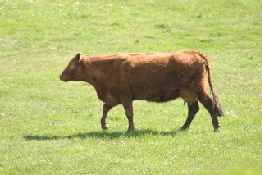
\includegraphics[width=4cm,keepaspectratio]{images/img.pdf}
    \quad
    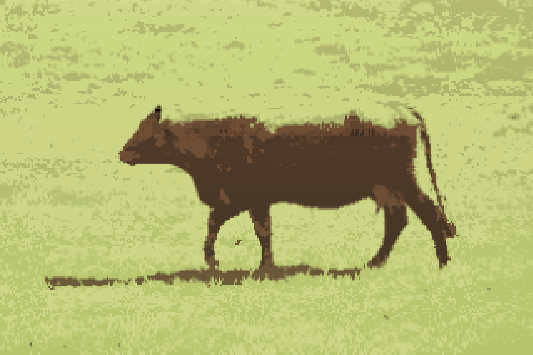
\includegraphics[width=4cm,keepaspectratio]{images/km.pdf}\\ \medskip
    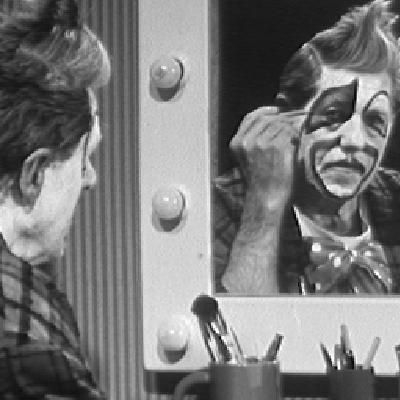
\includegraphics[width=4cm,keepaspectratio]{images/sobel.pdf}
    \quad
    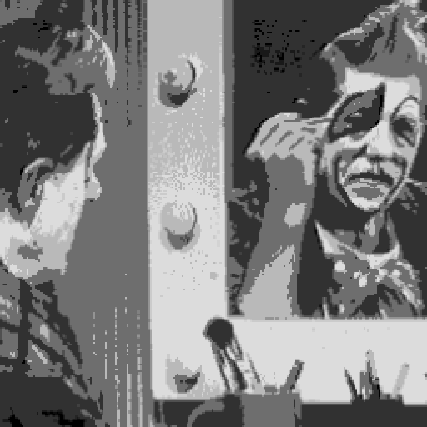
\includegraphics[width=4cm,keepaspectratio]{images/sobel_km.pdf}
  \end{center}
\end{frame}


\begin{frame}{Mean-shift}
  \begin{itemize}
    \item Využito pro segmentaci obrazu (3D barevný prostor RGB)
    \item Počet shluků je zvolen automaticky
    \item Bez optimalizací
    \medskip
    \item Jeden kernel pro každý bod obrazu X
    \medskip
      \begin{itemize}
        \item Vypočítá se střed (mean) S pro okno okolo X
        \item Přesune se okno tak, aby S bylo středem okna
        \item Pokud posunutí (shift) je větší než limit, iterujeme
      \end{itemize}
    \medskip
  \end{itemize}
\end{frame}


\begin{frame}{Mean-shift - ukázka výstupu}
  \begin{center}
    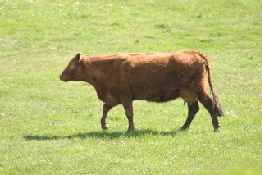
\includegraphics[width=4cm,keepaspectratio]{images/img.pdf}
    \quad
    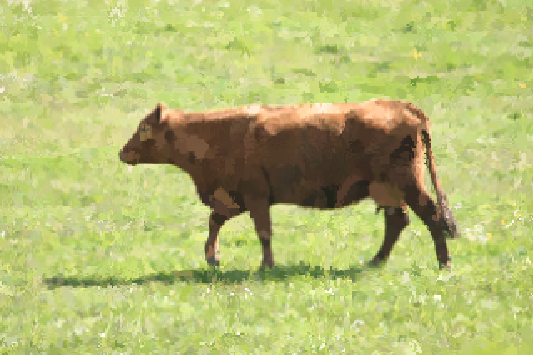
\includegraphics[width=4cm,keepaspectratio]{images/ms.pdf}\\ \medskip
    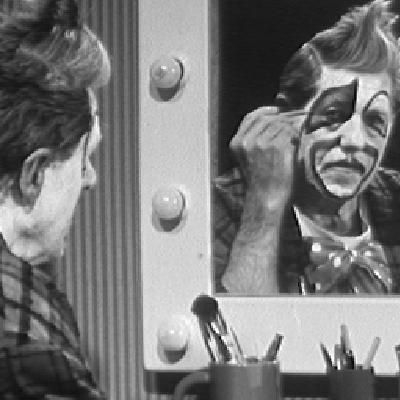
\includegraphics[width=4cm,keepaspectratio]{images/sobel.pdf}
    \quad
    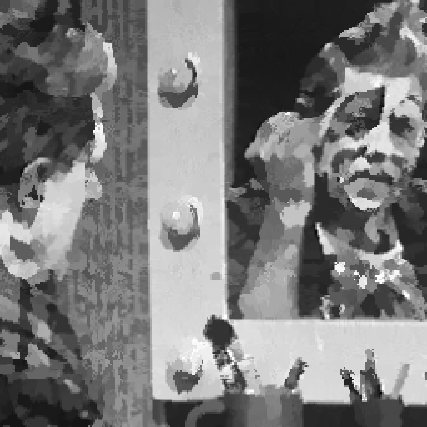
\includegraphics[width=4cm,keepaspectratio]{images/sobel_ms.pdf}
  \end{center}
\end{frame}


\begin{frame}{Závěr}
\begin{center}
    \begin{tabular}{| c | c | c | c | c | c | c |}
      \multicolumn{7}{ c }{K-means} \\
      \hline
      \tiny{Obrázek}   &  \tiny{K}  & \tiny{C2D E6850 (CPU)} & \tiny{i7 (CPU)} & \tiny{NV GT218M (GPU)} & \tiny{HD 4870 (GPU)} & \tiny{Akcelerace} \\
      \hline
      \tiny{512x512}   & \tiny{16}  &     \tiny{1.889 s}     &     \tiny{0.103 s}    &        \tiny{0.548 s}      &    \tiny{0.604 s}    & \tiny{X krát} \\
      \tiny{1920x1200} & \tiny{128} &    \tiny{13.688 s}     &     \tiny{5.655 s}    &        \tiny{N/A s}        &    \tiny{5.195 s}    & \tiny{X krát} \\
      \hline
    \end{tabular}
\end{center}
\begin{center}
    \begin{tabular}{| c | c | c | c | c | c | c |}
      \multicolumn{7}{ c }{Mean-shift} \\
      \hline
      \tiny{Obrázek} & \tiny{Okno}    & \tiny{C2D E6850 (CPU)} & \tiny{i7 (CPU)} & \tiny{NV GT218M (GPU)} & \tiny{HD 4870 (GPU)} & \tiny{Akcelerace} \\
      \hline
      \tiny{128x128} &   \tiny{25}    &      \tiny{1.837 s}    & \tiny{4.142 s}  &      \tiny{2.310 s}    &    \tiny{0.465 s}    & \tiny{X krát} \\
      \hline
    \end{tabular}
\end{center}
  \medskip
  \medskip
  \medskip
  
  \begin{center}
    Děkujeme za pozornost!\\
  %\end{center}
  \medskip
  %\begin{right}
    \textbf{Martin Šimon \& Pavel Širůček}
  \end{center}
\end{frame}


\end{document}
